\subsection{Background}
\paragraph{} 
Mr Snowden is a Physics Teacher at Northgate High School, teaching the subject at levels from KS3 to A-Level, there are also several other teachers in the department. During lessons, there are some times where it can be useful to the students to be able to see a model of the subject that they are learning about, while the majority of subjects that are taught have a range of models available, both real and software models. However one of the subjects where models are quite limited is in orbital mechanics and circular motion, with most being just simple animations and not a fully interactive or real-time simulation. The main disadvantage of this is that the students are not able to easily see how different modifications to a system will affect the outcome, something that can help to improve the understanding of a particular topic in some scenarios.

\subsubsection{Project Objective}
\paragraph{}
Mr Snowden requires a teaching tool that can provide a graphical sandbox to create and simulate various scenarios to fortify and replace the currently used tool-set of simple animations and power-point presentations that are used in teaching. This would allow the teacher in a physics lesson to quickly show students how a situation would develop, making use of SI units in order to effectively show students how different parameters (Mass, Size and Velocity) would affect a situation.

\subsubsection{Prospective Users}
\paragraph{}
While Mr Snowden is intended to be the primary user, other teachers could also have access to the tool as it could be put on the shared network drive, making the tool easy to access and used as a teaching aid in lessons, the tool will also be accessed by students, allowing the tool to be used as a revision resource for individual students on the school computers or at home. Because of this special attention should be paid to make sure that the program is as compatible as possible 

Because the users of the program are teachers and students (most likely A-Level) a good amount of technical knowledge in the field can be presumed, the tool will be used as a teaching aide, so it is not a requirement to explain the Physics in the program itself. It will be clear to anybody that studies Physics to a basic level what all the adjustment factors are.

\subsection{Current System}
\paragraph{}
The current system that is in place for teaching of orbital mechanics and in particular, newtons law of gravitation is mainly through the use of straight mathematical teaching, using the equations. Teachers will often write notes and examples for students to work through, past exam questions are also a popular choice.

\paragraph{}
Currently, simulation applets such as those found on the phET website are quite commonly used, these are mostly predefined animations with very few of them actually being true simulations.
Even the ones that are actual simulations are extremely limited and not particularly visually appealing. It is these tools that this project will aim to replace.

\paragraph{}
The main disadvantage with the phET tools is that their simulation is often not particularly accurate, one tool has a maximum of 4 bodies that it is able to simulate.

\paragraph{}
By having a application that has a very basic visual style, it will be a lot easier for a teacher to pause the simulation and annotate the board with extra information for students, such as going through a calculation in the current simulation state to prove the maths.

\subsection{Requirements and Processes}
\paragraph{}
The interface must be intuitive and self-explanatory in order to ensure that it is easy for teachers to understand, meaning that keyboard short-cuts should be ones that are commonly used in software (Such as $Ctrl-S$ for save) and any buttons should be clearly labelled. It must also be able to run well on the school computers, most of which are running on low end hardware (Dual-Core HT Intel i3 / Quad-Core Intel i5, ~2-4GB RAM) using a 32-Bit Windows operating system, as this is what all computers in the school are running for internal compatibility reasons. This applies a limit of 4GB to the total system RAM but a maximum per program usage of 2GB, meaning that the program will need to handle memory efficiently and potentially have a limit on the number of bodies (In the range of 1000s) to avoid using too much memory and causing the system to crash, a sensible limit would be 500MB. The number of bodies that this would support can be estimated however actual memory usage will likely be higher due to graphics library overhead, meaning that memory profiling should be used. The program must not require installation on the system or any secondary redistributes to be installed containing dynamic libraries.

\subsubsection{Graphics Processing}

\paragraph{}
While the resources of these systems are limited, keeping the program to being 2D should help to improve performance as there will be less demand on the integrated GPU (Graphics Processing Unit), meaning that it requires less system resources to display the simulation. This means that an external graphics library would need to be used in order to interface with this hardware and still function across different platforms. (The two main GPU Vendors, AMD and Nvidia, both have different interfaces for using GPUs for compute applications) 

\paragraph{}Having a 2D model also means that far less calculations need to be made for the simulation, making it faster, but it also reduces the load GPU in terms of rendering, As 3D would require shading and lighting to make depth perceivable. Input and camera movement would also be far more complex.

\subsubsection{Calculations and Trigonometry}
\paragraph{}
The application must be able to simulate the paths of at least three bodies, as this will encounter the n-body problem (n = Any positive integer), which in essence means that any interaction between two bodies can simply be predicted, however there is no direct solution for three or more bodies, and must be simulated through iterative process between each body to every other body.
The main calculation that will be used between bodies is:

$$F=\frac{Gm_1m_2}{d^2}$$

This calculation produces a result for the gravitational force between objects, taking into account the mass of the two planets and the distance between them, based on a universal gravitational constant. ($\num{6.67408e-11} m^{3} kg^{-1} s^{-2}$) 
While this equation only works between two bodies, the equation can be repeated in an iterative fashion in order to calculate the forces between all bodies in a system, the force can then be resolved to a single dimension for X and Y respectively, and then using a value for mass, acceleration can be calculated. By multiplying the acceleration by the change in time ($\Delta t$) of the simulation you can propagate a velocity ($v$) and change the position ($p$) of a body.

$$F_y=F\sin{\theta} \hspace{20pt} F_x=F\cos{\theta}$$

\paragraph{}
The main issue that could crop up is the computational cost of the trigonometric functions, while the instruction set used by processors in nearly all modern desktop computers (x86) has specific instructions for these functions.
The issue is that these still take longer than simple mathematical operators, which generally only take single instruction cycles. The difficulty is however that it will be heavily dependant both on the particular CPU running the code, but also the compiler used as well as the implementation used by the programming languages libraries.

\paragraph{}
There is also the issue that signs of calculated components to be flipped depending on which quadrant the simulated particle is in, adding further computational complexity. Trigonometric functions are also required to calculate the angle that the force is acting relative to the global X axis.

\paragraph{}
Because of these difficulties, it is worth investigating alternative methods for the calculation of the forces, as there could be far simpler methods that reduce the required complexity of code.

\subsubsection{Performance and Multithreading}

\paragraph{}
\textit{Since the Mid-2000s, CPU Clock speeds have all but stopped increasing in the consumer market, with most coming in at the 2GHz to 3GHz range. Some high end desktop processors are able to be effectively over-clocked, with processors like the AMD FX-9590 capable of 5GHz as long as adequate cooling is provided, the current world record is 8.794GHz, achieved by an AMD FX-8350, however this with with the use of Liquid Nitrogen to keep it cool.}

\paragraph{}
\textit{While clock speeds are effectively limited by the stability that can be achieved in the material being used (Silicon) and thermal properties, the focus has now switched to increasing the core count of CPUs, as well as improving their power efficiency and increasing their transistor count by shrinking the size of the transistors on die. (Consumer Intel CPUs are currently at 14nm, with 10nm on road map for 2017 and 5nm by 2021)}

\paragraph{}
\textit{Most Modern CPUs can be found with a core count of 2 or 4, with technologies such as hyper-threading allowing for multiple threads to be executed per core, effectively increasing the number of 'logical cores' by a factor of 2. High end desktop and workstation CPUs can be found with 6-12 physical cores, allowing for 12-24 consecutive threads. (Server CPUs are now coming with upwards of 18 physical cores, giving them 36 threads. These systems can also support multiple CPUs on the same motherboard, up to 8, allowing for effectively 288 consecutive threads on a single server.)}

\paragraph{}
Mutli-threading leads to is the potential to speed up the execution of the program by computing multiple parts of it at the same time. All of the computers in the school are new enough to have at a minimum dual core Intel i3 with hyper-threading, giving them a total of 4 'logical cores', this means that there is definitely some potential to improve the execution speed of the program.

\paragraph{} 
This opens up new challenges in the form of ensuring that the programming is \textit{'thread safe'}, this means that the program is not going to \textit{'step on its own toes'}, for example modifying data while another thread is reading it causing lock-ups, or race conditions where one thread completes a task before another and the program fails. When done properly the improvements to performance can be quite impressive.

\subsubsection{Saving of Scenarios}

\paragraph{}
The system will also need the ability to save the current scenario to a file, most likely a plain comma separated value file with a different file extension such as .sav, this will allow a teacher to set up a scenario inside the program outside of lesson time and save it for a future lesson, at which point it can be loaded into the program and used as a quick demo. These files could also be provided to students for use in their revision. Data for every body would need to be stored, namely Mass, Velocity and Position, constants could also be stored which would enable them to be changed in particular scenarios.

\subsubsection{Scale}

\paragraph{}
It is unlikely that true scale would translate particularly well to a program like this without visual aids added to the program, as distances are extremely massive, and planets are extremely small small in comparison to the sun, let alone the distances involved, for example, Earth has a diameter of only 12700 km, however it orbits the sun at a height of 150 Million km. At a zoom where both the sun and earth will be visible, the earth will be too small to make out, even on extremely high resolution monitors.

\subsection{Data Management}
\subsubsection{Data Sources and Destinations}
\import{tables/}{1_datasrcdest.tex}
% Data Sources and Destinations Table
\paragraph{}
Direct user input will be relatively low volume, taken in using keyboard short-cuts and mouse control, the user operates the program in order to place down objects, adjusting the initial size, mass and velocity of bodies in order to set-up the scenario, the user can also stop and start the program and change the speed of time within the simulation as well as other constants.

\paragraph{}
The loading and saving of scenarios will be sending and receiving similar data to what is provided by user inputs, however the data for an entire scenario will be transferred in one go, this includes the mass and size of bodies, as well as the most recent resolved (X, Y), Force, Velocity and Position of each simulated body, various constants that are set should also be stored, such as the gravitational constant, which can be changed by the user.

\paragraph{}
During the running of the simulation, the program will aim to keep the frame-rate (screen update) at 60 frames per second, (Ensures very smooth animation and responsiveness), this means that the data volumes during the running of the simulation are very high, as each frame could be a simulation update, this includes updating the resolved (X, Y) forces, velocity, acceleration and position of each body, according to how much simulation time passed per each frame.

\pagebreak

\subsubsection{Data Dictionary}
\paragraph{}
The main flow of data around the program will be body data, as there will need to be a container of some data type that will contain a large number of these bodies. Because this is a simulation, I want to make use of the common double data type, this is the IEEE Standard, 64 bit variable providing anywhere from 15-17 digits of precision depending on the specific hardware and software implementation used.

\paragraph{} 
While a float variable is smaller and only 32-Bits long, it is generally considered that there will be minimal computational benefit from using float instead of double on CPU bound simulations. In the majority of language mathematical functions take in double variables. While these can still take float variables, the operation will still performed as a double variable.

\paragraph{}
The double variable will also be useful for providing extra precision when it comes to the simulation variables, allowing the simulation to be potentially more accurate, however there may be situations where float can be beneficial to the memory footprint of the program.

\paragraph{}
It is also worth noting that if the simulation was being written to run on a GPU, the variables would need to be stored as floats unless a GPU with a large amount of double-precision units was being used as the target, as most GPUs will only have a small number of double-precision cores, often resulting in their performance being lower than what could be achieved using a CPU.

\paragraph{}
The variables written in the table below are likely to change as this project develops, particularly once the specific implementation is picked, things like program flow are more likely to develop during the programming stage.

\import{tables/}{2_datadictionary.tex}
% Data Dictionary Tables

\pagebreak

\subsubsection{Data Flow Diagrams}

\begin{figure}[!ht]
  \centering
  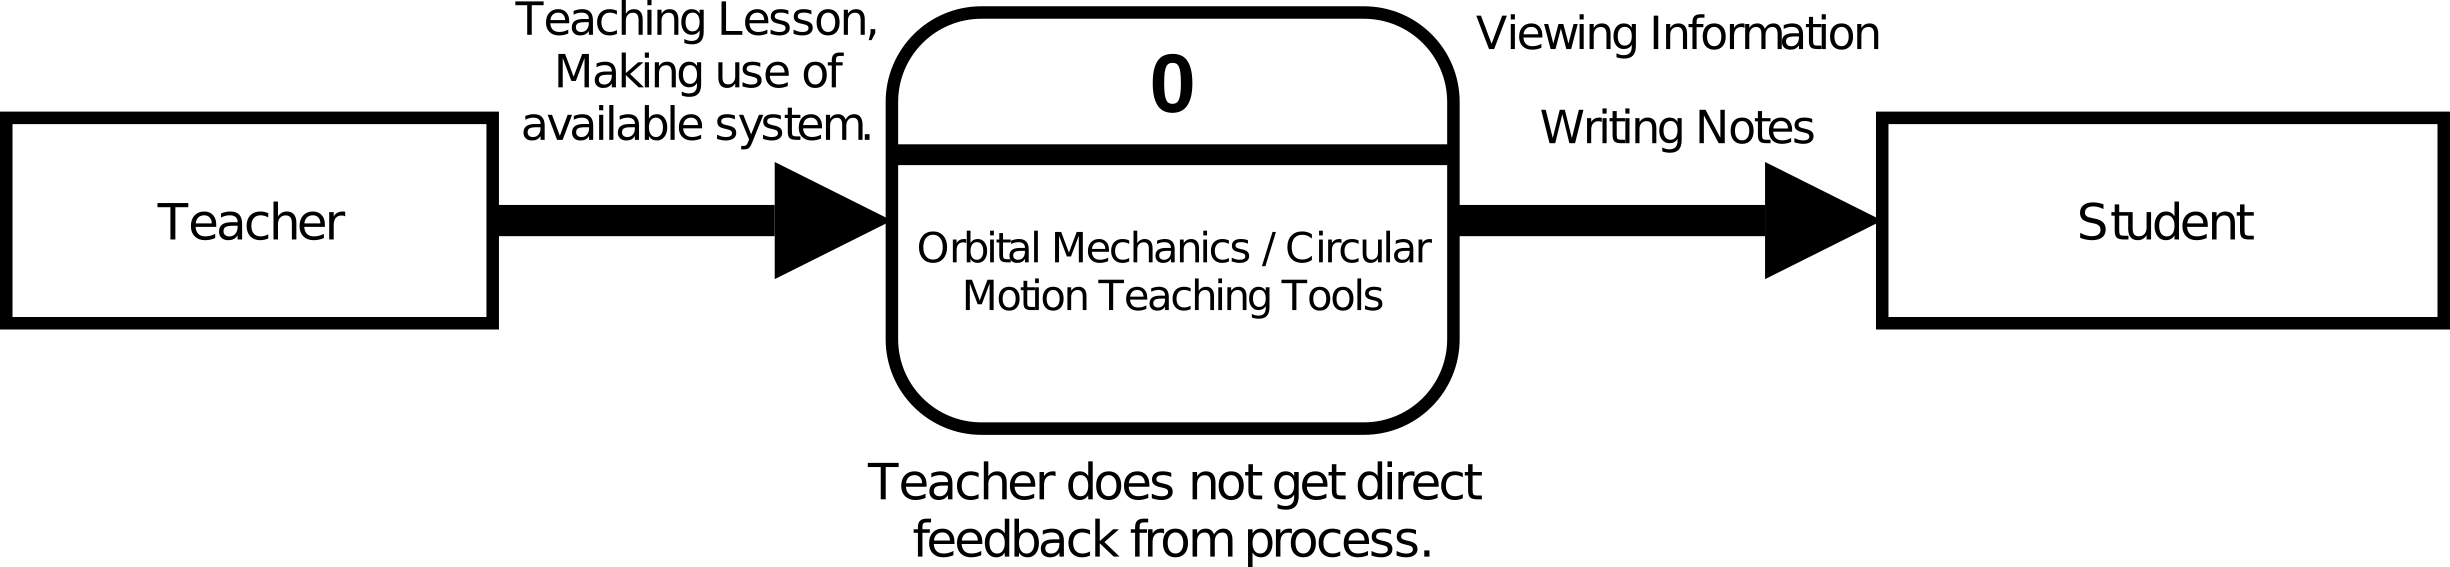
\includegraphics[width=\textwidth]{img/csl0.png}
  \caption{Current System, Level 0}
\end{figure}

\begin{figure}[!ht]
  \centering
  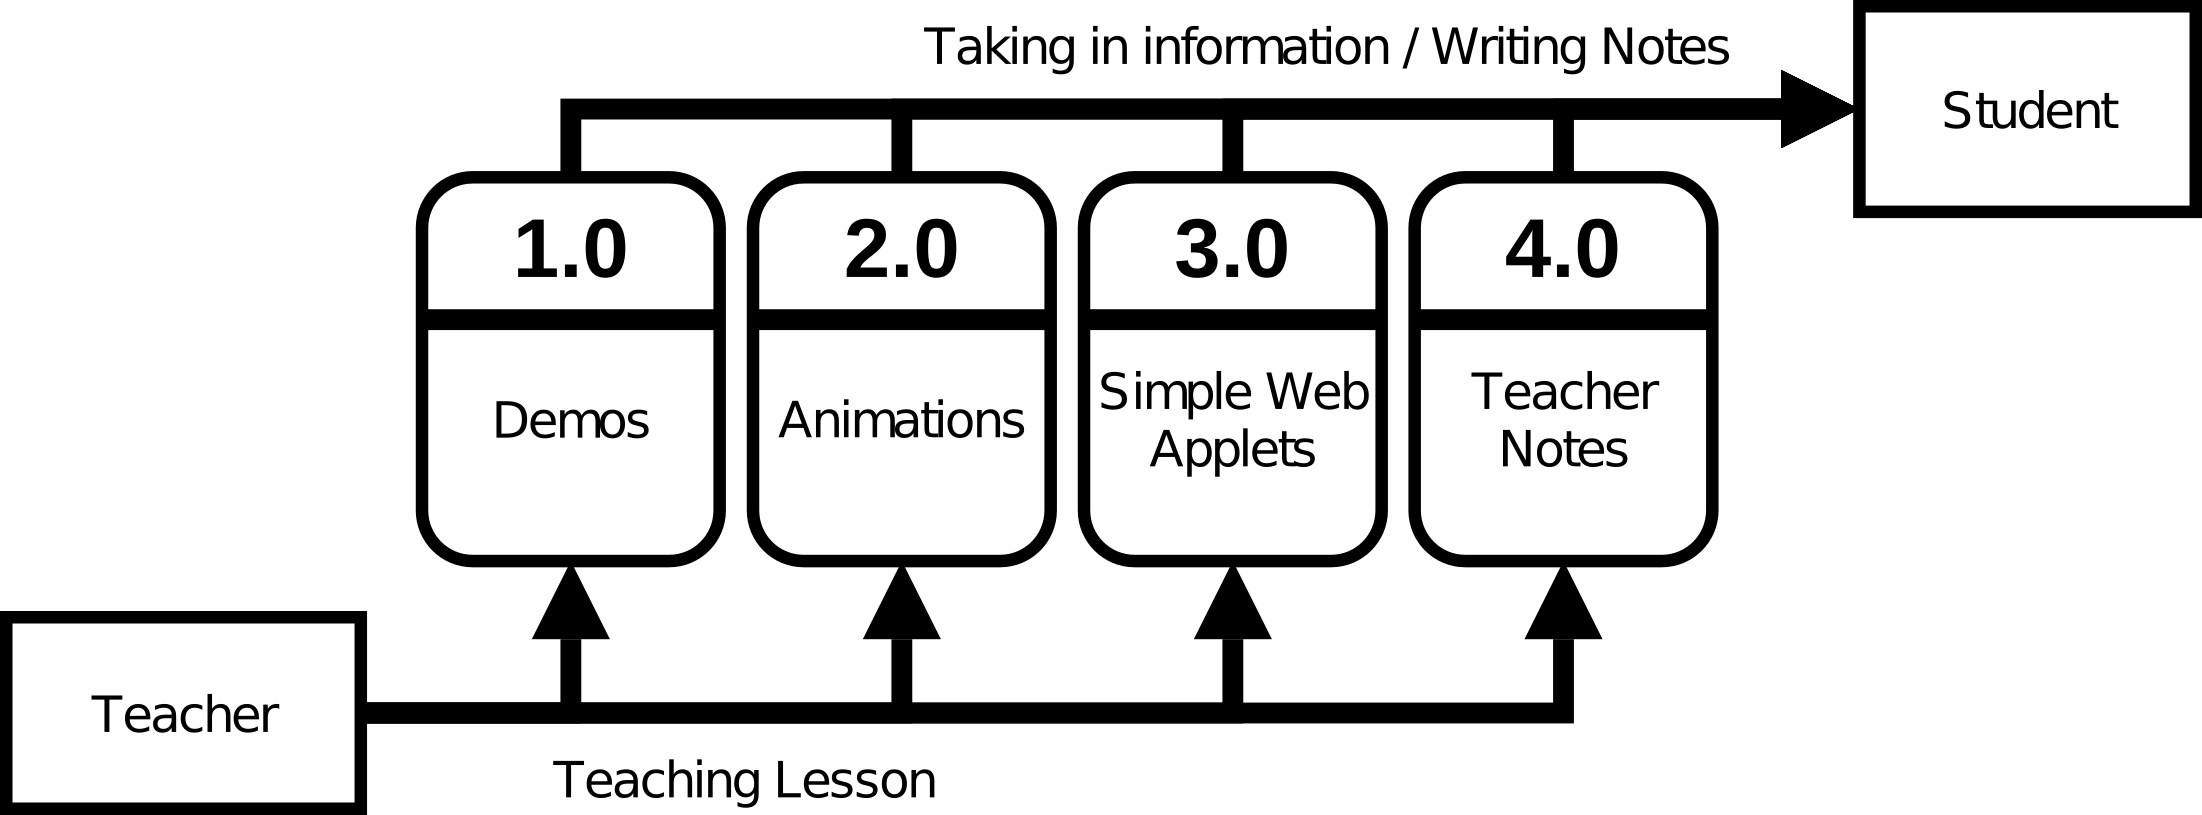
\includegraphics[width=\textwidth]{img/csl1.png}
  \caption{Current System, Level 1}
\end{figure}

\begin{figure}[H]
  \centering
  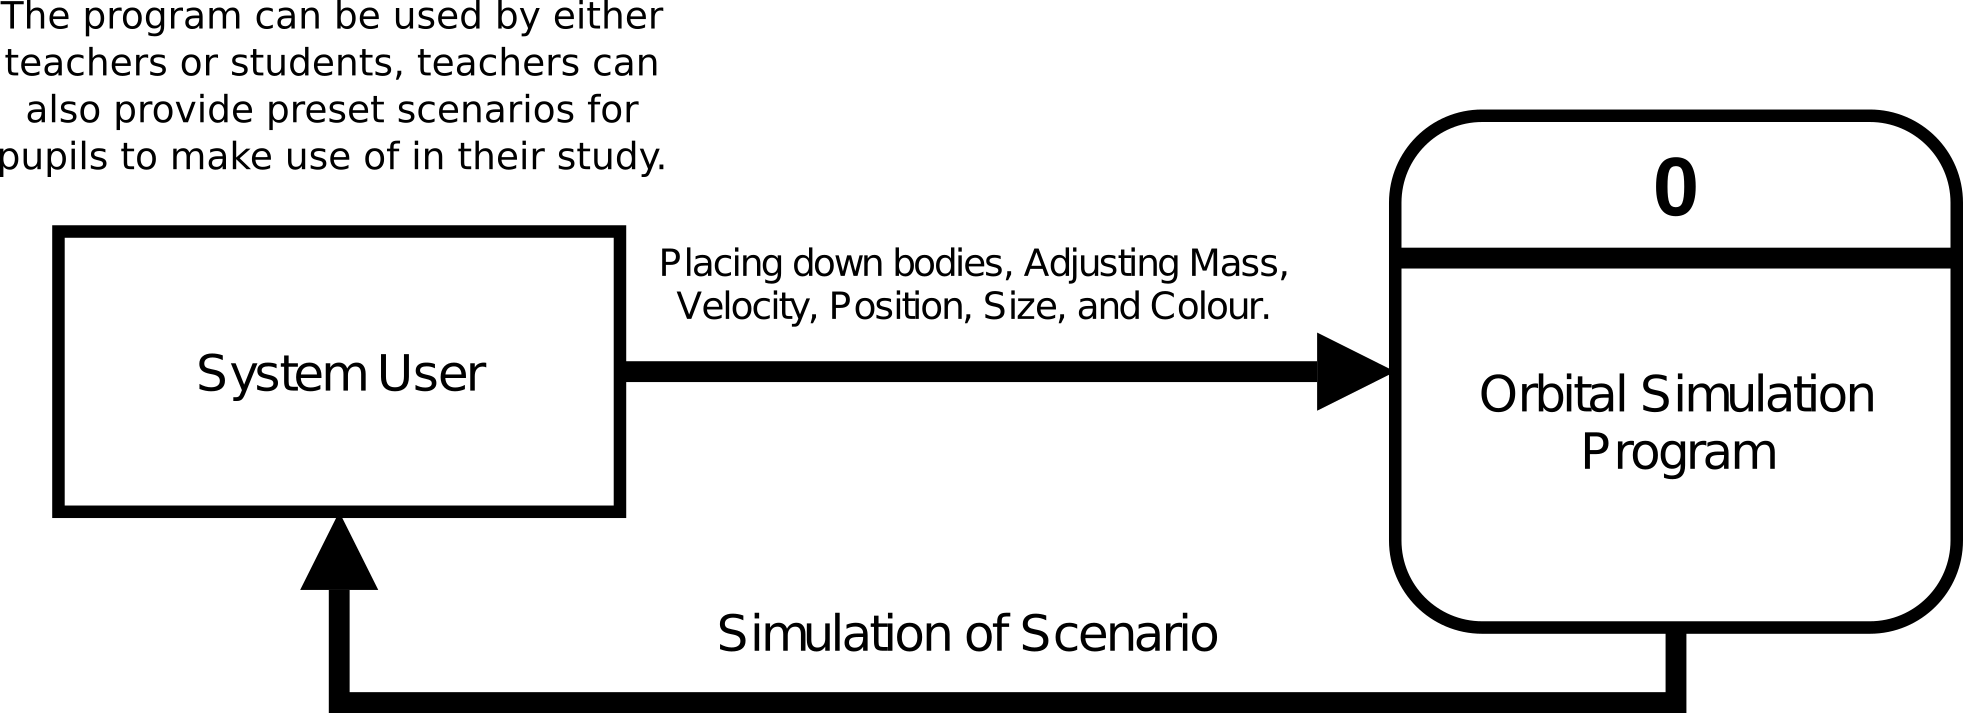
\includegraphics[width=\textwidth]{img/nsl0.png}
  \caption{New System, Level 0}
\end{figure}

\begin{figure}[!ht]
  \centering
  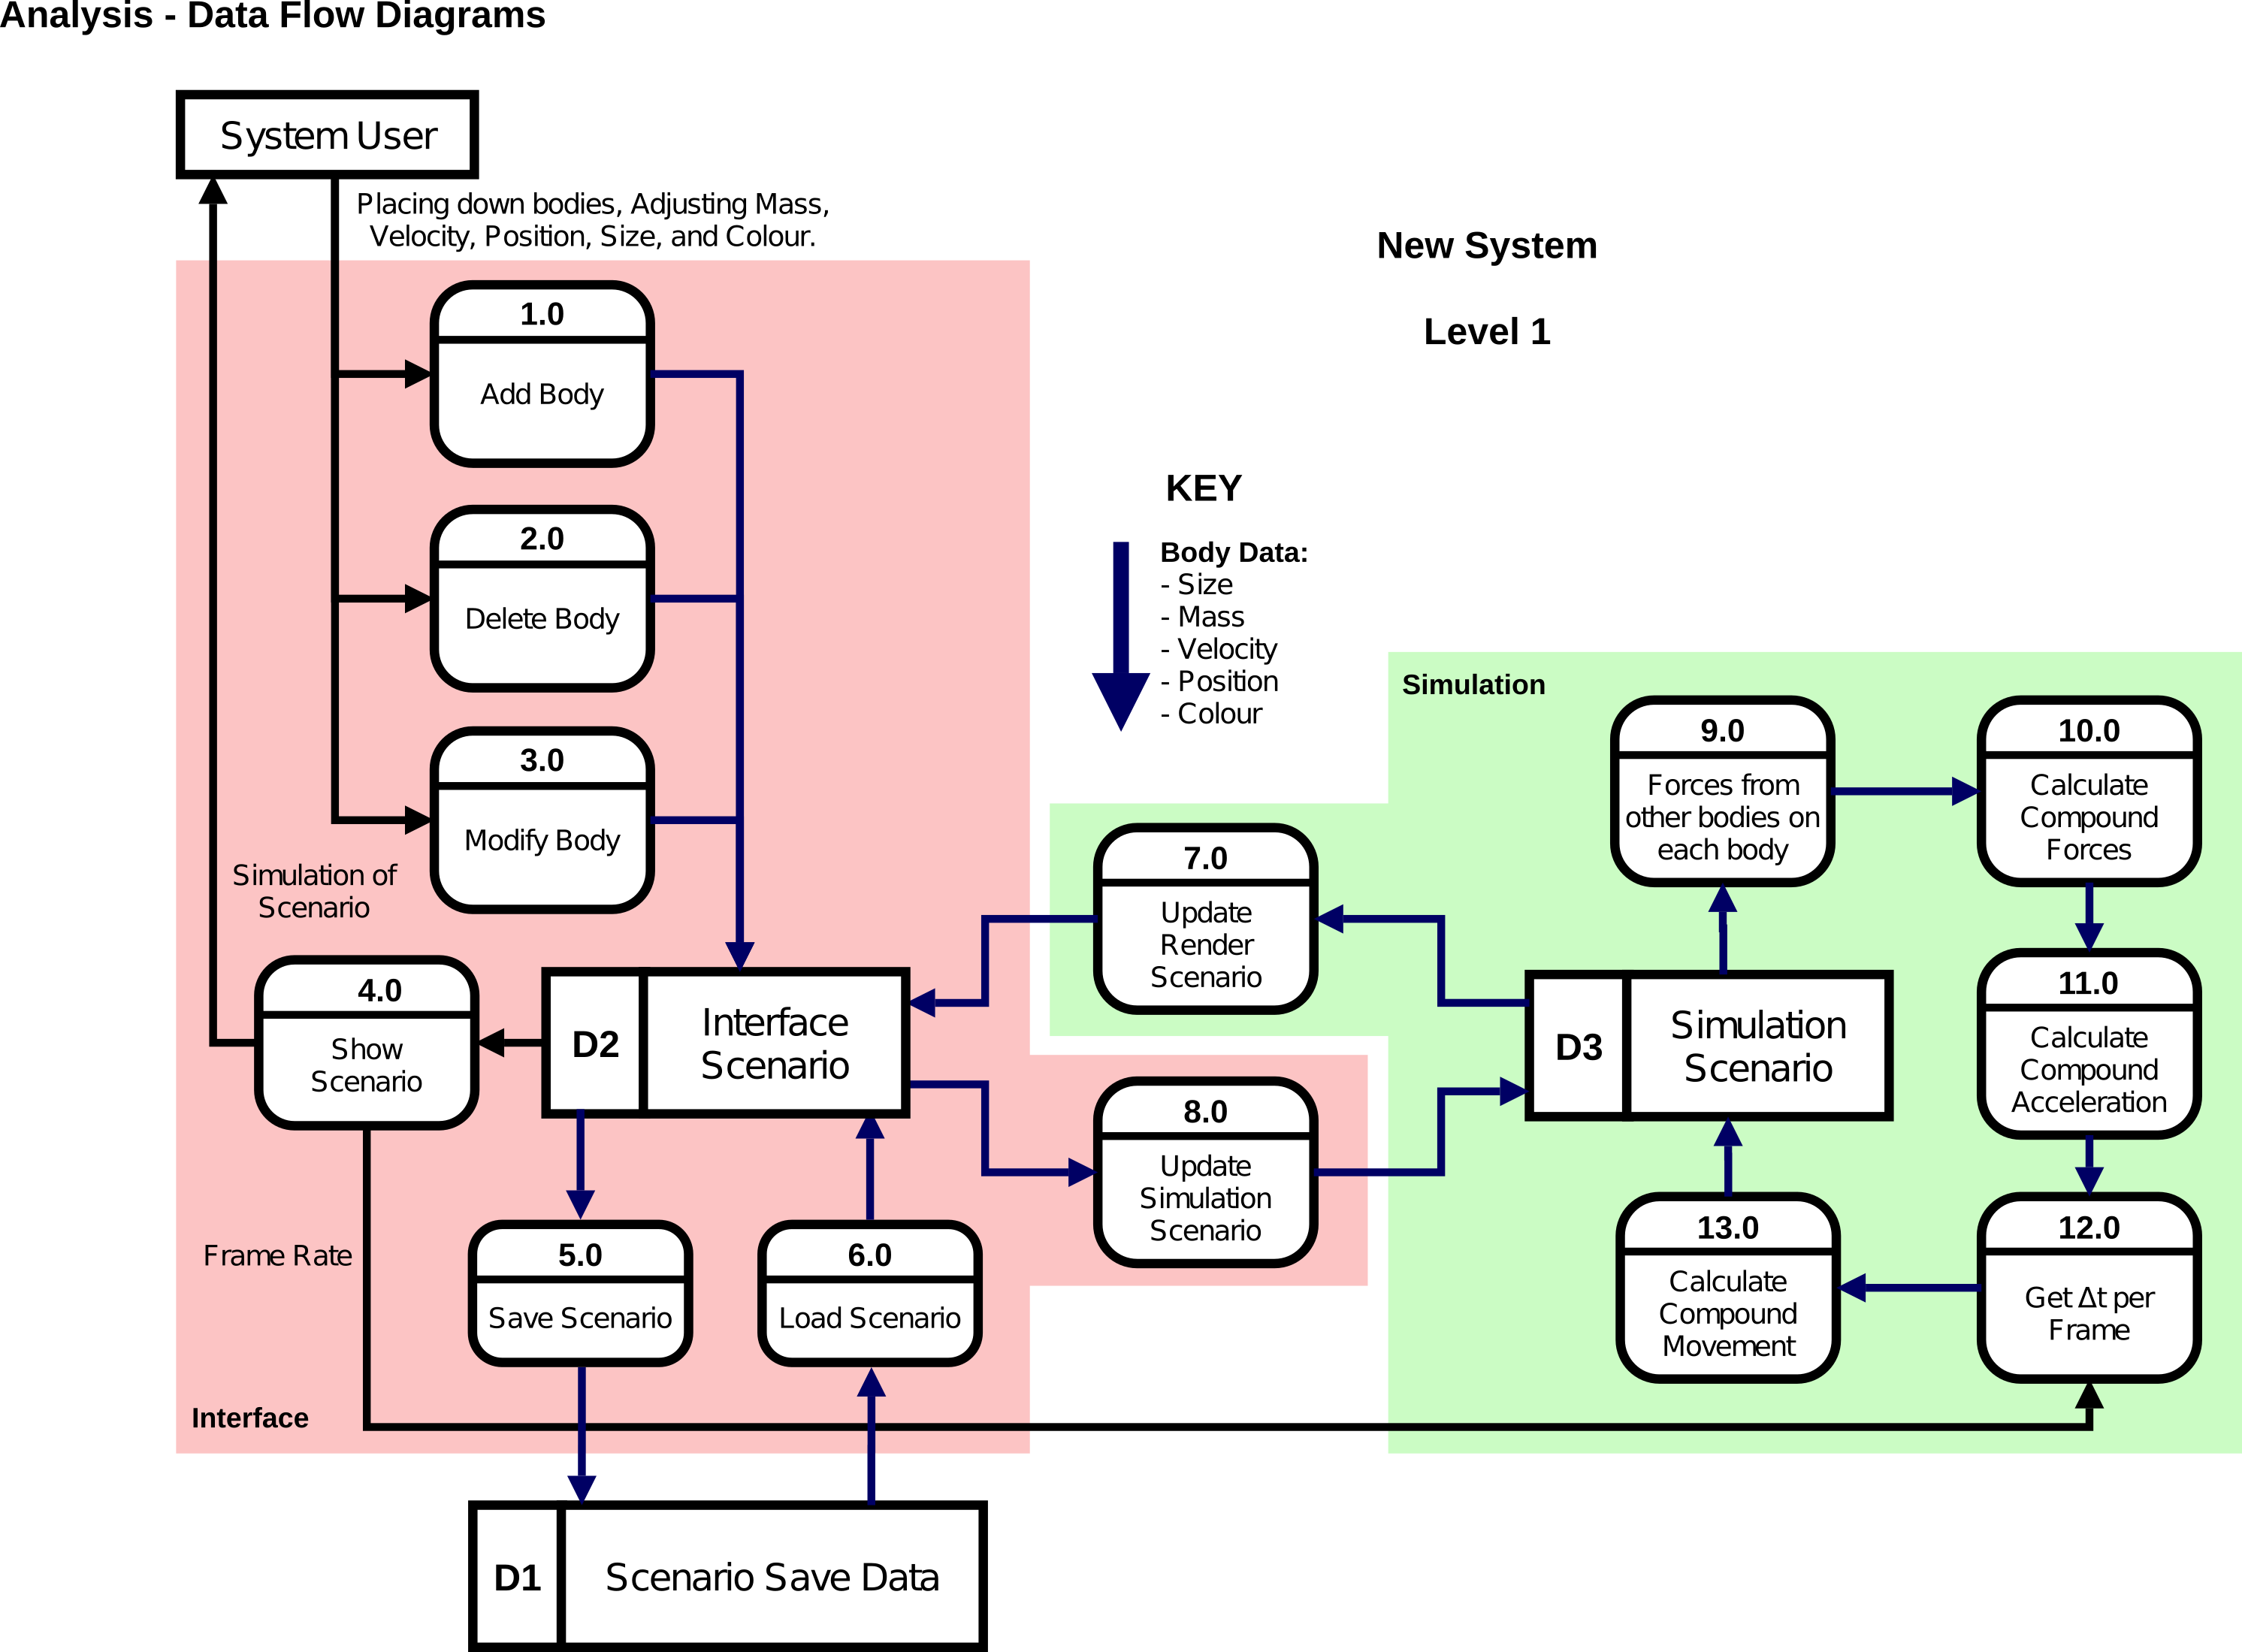
\includegraphics[angle=-90, width=0.99\textwidth]{img/nsl1.png}
  \caption{New System, Level 1}
\end{figure}

\subsection{Limitations}
\paragraph{}
When it comes to limitations, the main one to consider will be the dimensions of the simulation, while it would be relatively straightforward to program a 3D simulation, it would increase the computational requirement for the program as well as make the rendering far more complex, requiring some form of lighting and shading calculations to make the display useful in any way.

\paragraph{}
The disadvantage of having a more complicated visual display is that it will be much easier to miss displayed information on the screen, particularly from the view of students. This is because the teacher will likely be projecting the application onto the whiteboard, due to the nature of the projectors they don't produce the best quality image and often struggle with contrast, having complex shading would just serve to make matters worse.

\paragraph{}
The system being used is as mentioned previously something of a brute force method, while more efficient algorithms exist, such as Barnes-Hut I do not plan on implementing these, as they are more suited to extremely large simulations with hundreds of thousands to hundreds of billions of bodies over galactic scales. Often these are implemented on supercomputer clusters.

\subsection{Objectives}
\import{sections/analysis/}{objectives.tex}

\subsection{User Dialogue}
\paragraph{}
Email correspondence with the user can be found in Appendix A.

\pagebreak
\subsection{Potential Solutions}
\import{sections/analysis/}{solutions.tex}

\pagebreak
\subsection{Management and Tools}
\subsubsection{Linux and Development Environment}
\paragraph{}
When it comes to the management and writing of the code, I will be using a bare-bones text editor with auto-complete plug-ins to make the experience somewhat smoother. A custom makefile will be used in order to create a custom build system which will make building an application with multiple source and header files much easier.

\paragraph{}
I plan on using the Linux operating system for the main development of the program, the main reason for this is that there are several tools that integrate very well into the Linux environment. As well as this, build tools and compilers are generally far better supported and more up to date on Linux.

\paragraph{}
In order to improve the organisation of code, different files will be split into separate directories source files will be found in $src/$, header files in $include/$, compiled object (.o) files will stored in $bin/$.
Having .o files in a separate directory means that the files can be kept after the program is linked, if any change is made to a particular source file only that file needs to be recompiled and the older files can just be linked together to produce a new executable.

\paragraph{}
Because I will be developing the software using Linux, I will need to work out an alternative build system to build an executable binary for Windows. It is possible to do this from within the Linux Environment. (e.g: CMake)

\subsubsection{Git - Version Control}
\paragraph{}
I will make use of tools such as \textit{Git} (Originally written by Linus Torvalds, Creator of Linux) for the management and version control of the source code, this allows me to make changes to my code and upload it to a remote server. The code can be 'pulled' on other computers, changes can be 'staged' and 'committed', the resulting 'commits' can then be 'pushed to the remote server. Git provides options to split changes to code into separate branches for making experimental changes to the code without making changes to the 'master' code.

\paragraph{}
Another feature of Git is the ability to automatically merge code, if a multiple changes are made to code on different computers (Such as forgetting to pull changes from remote.) the modified code can be staged to a commit and the previous remote commit can be pulled from the server. Git will then attempt to automatically merge the code together in a way that preserves its function. (In the case that it cannot, it presents differences to you and asks you to merge the code manually.)

\paragraph{}
It is possible to completely revert code back to any previously commit, all of these features make Git and invaluable tool for the maintenance of source code, even for small project. (It make working on collaborative projects far easier also.) The fact that code is stored on an external server is an added bonus as it provides an off site backup and makes it possible to access code anywhere with an internet connection, but still make changes and commits to a local copy without a connection.

\subsubsection{GDB - Debugging}
\paragraph{}
The GNU Debugger is an invaluable tool for the 'real-time' debugging of applications, assuming that the application has debugging symbols compiled in it is possible to run through code line by line stepping through code.

\paragraph{}
The tool allows individual variables to be looked at, allowing you to check that the program is running as intended. It will also return more information in the event of exceptions.

\paragraph{}
The main disadvantage to this tool is that even when the program is set to continuously run, it will run at a much lower speed than the program running outside the tool would run at, making this not a tool for profiling the performance of the application.

\subsubsection{Valgrind - Profiling and Memory Analysis}
\paragraph{}
Valgrind is a tool which can be used for profiling certain aspects of the programs runtime, mainly looking at the programs use of memory.

\paragraph{}
The tool will print errors to a terminal in the case that it detects programming that could potentially be causing memory leaks to occur. After the program finishes or is exited the tool will print the total memory usage at the end of the program, it will also print out its analysis of potentially lost memory.

\paragraph{Included Tools}
\begin{itemize}
\item Memcheck - Memory error detector \footnotemark[1]
  \begin{itemize}
  \item Illegal Access
  \item Undefined Variables
  \item Incorrect Memory Management
  \item Overlapping Allocation
  \item Negative Memory Sizes
  \item Memory Leaks
  \end{itemize}
\item Cachegrind - Cache Interaction Simulator
\item Callgrind - Call Profiling Tool \footnotemark[1]
  \begin{itemize}
  \item Function Calls
  \item Function 'Cost'
  \item Includes Cache Simulator - Cachegrind
  \item Other Events
  \end{itemize}
\item Helgrind - Multi-thread Synchronisation \footnotemark[1]
\item DRD - Multi-threading Errors \footnotemark[1]
\item Massif - Heap Profiler \footnotemark[1]
  \begin{itemize}
  \item Memory Usage
  \item Stack Usage
  \item Long Term Leaks
  \end{itemize}
\item DHAT - Heap Allocation \footnotemark[2]
\item SGCheck - Stack and Global Array Overrun
\item BBV - Basic Block Vector \footnotemark[2]
\end{itemize}

\footnotetext[1]{Will Use}
\footnotetext[2]{May Use}



























































